\documentclass[11pt, a4paper]{article}
\usepackage{polski}
\usepackage[utf8]{inputenc}
\usepackage[T1]{fontenc}
\usepackage[export]{adjustbox}
\usepackage{graphicx}
\usepackage{amsmath} 
\usepackage{listings}
\usepackage{color}
\usepackage{marvosym}
\usepackage{geometry}
\usepackage{float}
\usepackage{booktabs}
\usepackage{multirow}
\usepackage{titlesec}
\usepackage{hyperref}
\usepackage{tabularx}

\geometry{margin=1.2in}
\usepackage[final]{pdfpages}

\newcommand{\fbi}{\leavevmode{\parindent=1em\indent}}

\definecolor{dkgreen}{rgb}{0,0.6,0}
\definecolor{gray}{rgb}{0.5,0.5,0.5}
\definecolor{mauve}{rgb}{0.58,0,0.82}

\lstset{
	frame=tblr,
	language=R,
	aboveskip=3mm,
	belowskip=3mm,
	showstringspaces=false,
	columns=flexible,
	basicstyle={\small\ttfamily},
	numbers=left,
	numberstyle=\tiny\color{gray},
	keywordstyle=\color{blue},
	commentstyle=\color{dkgreen},
	stringstyle=\color{mauve},
	breaklines=true,
	mathescape=false,
	breakatwhitespace=true,
	tabsize=3
}

\renewcommand\lstlistingname{Listing}

\titleclass{\subsubsubsection}{straight}[\subsection]
\newcounter{subsubsubsection}[subsubsection]
\renewcommand\thesubsubsubsection{\thesubsubsection.\arabic{subsubsubsection}}
\renewcommand\theparagraph{\thesubsubsubsection.\arabic{paragraph}}

\titleformat{\subsubsubsection}
  {\normalfont\normalsize\bfseries}{\thesubsubsubsection}{1em}{}
\titlespacing*{\subsubsubsection}
{0pt}{3.25ex plus 1ex minus .2ex}{1.5ex plus .2ex}

\makeatletter
\renewcommand\paragraph{\@startsection{paragraph}{5}{\z@}
  {3.25ex \@plus1ex \@minus.2ex}
  {-0em}
  {\normalfont\normalsize\bfseries}}
\renewcommand\subparagraph{\@startsection{subparagraph}{6}{\parindent}
  {3.25ex \@plus1ex \@minus .2ex}
  {-1em}
  {\normalfont\normalsize\bfseries}}
\def\toclevel@subsubsubsection{4}
\def\toclevel@paragraph{5}
\def\toclevel@paragraph{6}
\def\l@subsubsubsection{\@dottedtocline{4}{7em}{4em}}
\def\l@paragraph{\@dottedtocline{5}{10em}{5em}}
\def\l@subparagraph{\@dottedtocline{6}{14em}{6em}}
\makeatother

\setcounter{secnumdepth}{4}
\setcounter{tocdepth}{4}

\hypersetup{pageanchor=false}

\setlength\parindent{3pt}

\renewcommand{\labelenumi}{\alph{enumi}.} 

\date{\today}

\begin{document}

\begin{titlepage}

\newcommand{\HRule}{\rule{\linewidth}{0.5mm}} 
\center 

\textsc{\LARGE Politechnika Wrocławska}\\[1.5cm] 
\textsc{\Large Inteligencja Obliczeniowa i jej zastosowania}\\[0.5cm] 
\HRule \\[0.5cm]
{ \huge \bfseries Badanie algorytmu genetycznego z zakresu optymalizacji globalnej dla wybranych funkcji testowych}\\[0.5cm] 
\HRule \\[1.6cm]
 
\begin{minipage}{0.4\textwidth}
\begin{flushleft} \large
\emph{Autorzy:}\\
Paweł  \textsc{Andziul} 200648 \\
Marcin  \textsc{Słowiński} 200638 \\
\end{flushleft}
\end{minipage}
~
\begin{minipage}{0.4\textwidth}
\begin{flushright} \large
\emph{Prowadzący:} \\
dr hab. inż. Olgierd \textsc{Unold}, prof. nadzw. PWr
\end{flushright}
\end{minipage}\\[4cm]

\vfill 
{\large 5 kwietnia 2017}\\[3cm] 

\end{titlepage}

\tableofcontents

\newpage
\section{Wprowadzenie}
\paragraph{}
Algorytm genetyczny – algorytm heurystyczny, który swoim działaniem przypomina działanie ewolucji w~naturze. Osobniki będące zbyt słabe zostają wyeliminowane z~populacji w~kolejnych pokoleniach, a~na ich miejsce przyjmowane są lepsze, silniejsze, bardziej adaptowalne. Algorytmy te zakładają możliwość mutacji i~krzyżowania wśród potomków, przez co nie zawsze są oni silniejsi od poprzednio wyeliminowanych członków. Dodatkowo wprowadzają pojęcie elity, która jest bezpośrednio przenoszona do następnego - teoretycznie lepszego pokolenia.

\fbi
W ramach laboratorium należało przeprowadzić testy algorytmu genetycznego dla różnych parametrów. Jako benchmark oceny należało użyć pakietu ,,getGlobalOpts'' oraz języka R.

\fbi
Pomiary wykonywano na 2 różnych jednostkach roboczych. Ich parametry nie są istotne z~punktu widzenia analizy i~możliwości porównania rezultatów.

\section{Implementacja}
\paragraph{}
Poniżej (listing ~\ref{lst:skryptGlowny}) zamieszczono kod napisany w~języku R przygotowany w~celu umożliwienia przeprowadzenia pomiarów.

\lstinputlisting[label=lst:skryptGlowny,caption=Skrypt w~języku R wykorzystany do badań,firstline=1,lastline=300]{./assets/skrypt_lab12.R}

\fbi
Skrypt przygotowano w~sposób który umożliwia w~pełni automatyczne przeprowadzenie wszystkich pomiarów. Jednocześnie wszystkie wykresy mogą być natychmiast podmienione w~sprawozdaniu. Poniżej pokrótce omówiono podstawowe parametry.

\begin{itemize}
	\item nOfRuns
	
	Ilość powtórzeń dla każdego pomiaru w~celu uśrednienia.
	
	\item colors, series
	
	Wektory kolorów i~nazw kolejnych serii pomiarowych. 
	
	\item params
	
	Macierz parametrów domyślnych algorytmu dla każdej z~serii. W każdym wierszu kolejno są zawarte: p. mutacji, p. krzyżowania, rozmiar populacji, ilość iteracji oraz kolor serii na wykresach.
	
	\item functions
	
	Wektor nazw funkcji dla których przeprowadzane są kolejno pomiary.
	
\end{itemize}

Całość informacji niezbędnych do przeprowadzenia obliczeń odczytywana jest na podstawie nazwy funkcji z~pakietu ,,globalOptTests''. Są to: rozmiar problemu (ilość parametrów), domyślne ograniczenia, wartość w~danym punkcie oraz optimum dla domyślnych ograniczeń.

\newpage
\section{Przebieg badań}
\paragraph{}
Do badań zostały wybrane funkcje o~różnych wymiarach zaczynając na 2 kończąc na 20. Poniżej wymieniono te funkcje wraz z~ilością wymiarów podaną w~nawiasie.

\begin{itemize}
	\item Branin (2)
	\item Gulf (3)
	\item CosMix4 (4)
	\item EMichalewicz (5)
	\item Hartman6 (6)
	\item PriceTransistor (9)
	\item Schwefel (10)
	\item Zeldasine20 (20)
\end{itemize}

\fbi
Każdy pomiar przeprowadzono 20-krotnie wyniki uśredniając co oznacza, że wartości widoczne na wykresach dla każdej serii z~osobna są uśrednione po osobnych 20 przebiegach. Domyślne parametry każdej z~serii przedstawiono poniżej (tabela~\ref{tab:parametry}). Zmianie ulegają wartości  prawdopodobieństwa mutacji i~krzyżowania by zbadać znaczenie ich obecności podczas optymalizacji.

\begin{table}[H]
	\centering
	\caption{Parametry domyślne poszczególnych serii pomiarowych}
	\label{tab:parametry}
	\begin{tabularx}{\textwidth}{|X|c|c|c|c|}
		\hline
		- & Seria 1 & Seria 2 & Seria 3 & Seria 4\\ 
		\hline
		Rozmiar populacji & 50 & 50 & 50 & 50 \\ 
		\hline 
		Rozmiar iteracji & 100 & 100 & 100 & 100 \\ 
		\hline 
		Prawdopodobieństwo mutacji & 0 & 0 & 0.1 & 0.1 \\ 
		\hline 
		Prawdopodobieństwo krzyżowania & 0 & 0.8 & 0 & 0.8 \\ 
		\hline 
	\end{tabularx} 
\end{table}

\fbi
Zielone linie na wykresach oznaczają optima zawarte w~pakiecie ,,globalOptTests'' dla danej funkcji przy domyślnych ograniczeniach (tych samych dla których wykonywana jest optymalizacja podczas niniejszych pomiarów).

\fbi
Dla funkcji o~ilości parametrów większej niż 2 pominięto ilustracje graficzne znalezionych optimów gdyż optymalizacji podlegają wszystkie wymiary. Ilustracja dla dwóch pierwszych nie niesie ze sobą przydatnej informacji.

\newpage
\subsection{Branin (2 parametry)}
\paragraph{}
Branin jest funkcją z~dwoma parametrami. Na ilustracji (rys.~\ref{fig:branin1}) przedstawiono jej wykres a~poniżej jej wzór (\ref{eq:branin}).

\begin{equation}\label{eq:branin}
	f(\boldsymbol{x}) = a(x_2 - bx_1^2 + cx_1 - r)^2 + s(1 - t)\cos(x_1) + s
\end{equation}

, gdzie $ x_1 \in [-5, 10] $ oraz $ x_2 \in [0, 15] $.

\begin{figure}[H]
	\centering
	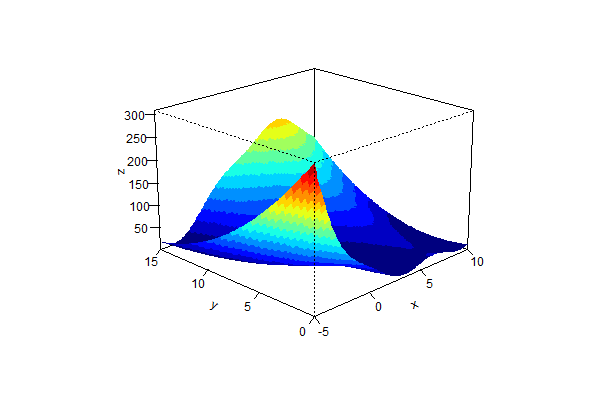
\includegraphics[width=0.95\textwidth]{./assets/Branin1.png}
	\caption{Wykres funkcji Branin}
	\label{fig:branin1}
\end{figure}

\fbi
Z wykresu (rys.~\ref{fig:branin1}) wynika, że funkcja ta ma stosunkowo duży obszar w~którym może znajdować się minimum oraz dwie strefy w~których wartości są dużo większe.

\fbi
Na kolejnych stronach zamieszczono wyniki pomiarów dla różnych wartości parametrów algorytmu genetycznego. Kolejno dokonano pomiarów dla różnych wartości: prawdopodobieństwa mutacji i~krzyżowania, wielkości populacji, ilości iteracji oraz elityzmu. Wszystkie pomiary wykonano dla 4 różnych ustawień domyślnych parametrów (serie 1 -- 4).

\newpage
\begin{figure}[H]
	\centering
	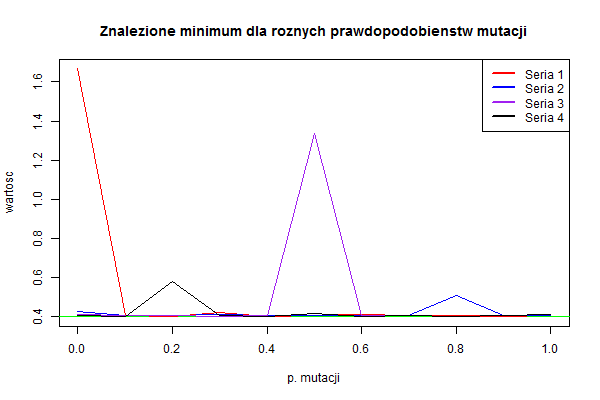
\includegraphics[width=0.85\textwidth]{./assets/Branin2.png}
	\caption{Wartość znalezionego minimum funkcji Branin w~zależności od prawdopodobieństwa mutacji}
	\label{fig:branin2}
\end{figure}

\begin{figure}[H]
	\centering
	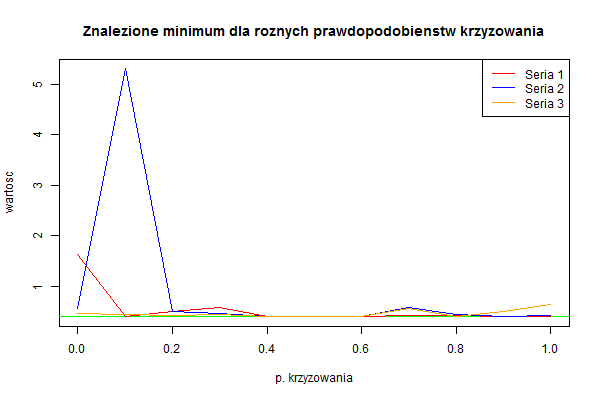
\includegraphics[width=0.85\textwidth]{./assets/Branin3.png}
	\caption{Wartość znalezionego minimum funkcji Branin w~zależności od prawdopodobieństwa krzyżowania}
	\label{fig:branin3}
\end{figure}

\fbi
Na wykresie (rys.~\ref{fig:branin2}) można zauważyć niski wpływ ustawienia mutacji na znalezione rozwiązania. Przy wszystkich parametrach domyślnych funkcja znajduje się w~pobliżu optymalnej wartości. Miejscowe odchylenia są tu najprawdopodobniej związane z~charakterem algorytmu i~zbyt małą ilością prób poddanych uśrednieniu. Nie możemy tutaj określić czy przy wyłączonej zarówno mutacji jak i~krzyżowaniu wyniki ulegają pogorszeniu, gdyż nie ma w~tym obszarze spójności. Podobne wnioski możemy wskazać dla wykresu krzyżowania (rys.~\ref{fig:branin3}).

\begin{figure}[H]
	\centering
	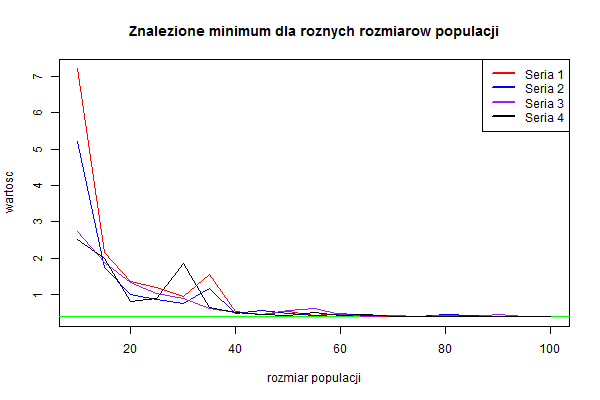
\includegraphics[width=0.85\textwidth]{./assets/Branin4.png}
	\caption{Wartość znalezionego minimum funkcji Branin w~zależności od rozmiaru populacji}
	\label{fig:branin4}
\end{figure}

\begin{figure}[H]
	\centering
	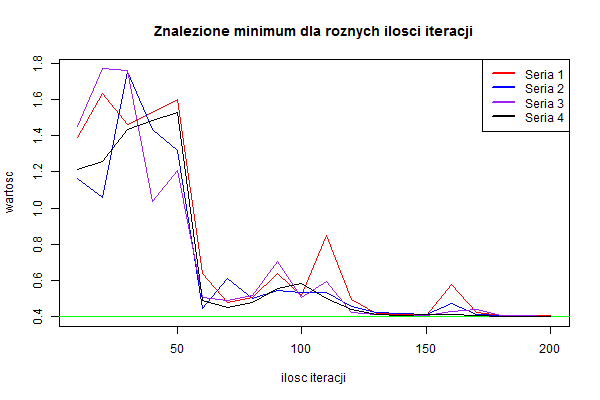
\includegraphics[width=0.85\textwidth]{./assets/Branin5.png}
	\caption{Wartość znalezionego minimum funkcji Branin w~zależności od ilości iteracji}
	\label{fig:branin5}
\end{figure}

\fbi
Z wykresu (rys.~\ref{fig:branin4}) można odczytać podatność funkcji na zmiany rozmiaru populacji. Wyniki zbliżone do oczekiwanych zostały uzyskane dla wartości wynoszącej 45 jednostek. Widać również, że przy małej populacji znaczenie mutacji i~krzyżowania jest większe. Zauważalny jest wzrost jakości rozwiązania wraz ze wzrostem ilości jednostek populacji.

\fbi
Wykres (rys.~\ref{fig:branin5}) wskazuje wyraźną zmianę jakości rozwiązań dla 60 i~więcej iteracji. Poniżej tej wartości uzyskiwane wyniki są niestabilne, powyżej osiągają wartość zbliżoną do oczekiwanej szczególnie dla serii 4 (czyli z~włączoną mutacją i~krzyżowaniem).

\begin{figure}[H]
	\centering
	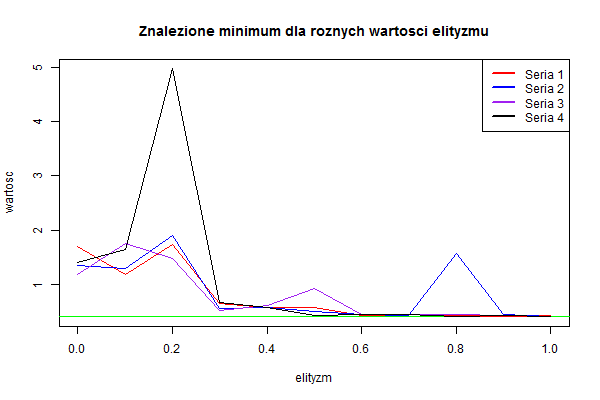
\includegraphics[width=0.85\textwidth]{./assets/Branin6.png}
	\caption{Wartość znalezionego minimum funkcji Branin w~zależności od przyjętego elityzmu}
	\label{fig:branin6}
\end{figure}

\fbi
Z wykonanych pomiarów (rys.~\ref{fig:branin6}) wynika, że dla uzyskania optymalnego rozwiązania należy zastosować wartość elityzmu na poziomie przynajmniej 0.4. Jego ustawienie poniżej tej wartości powoduje obniżenie się jakości rezultatów.

\begin{figure}[H]
	\centering
	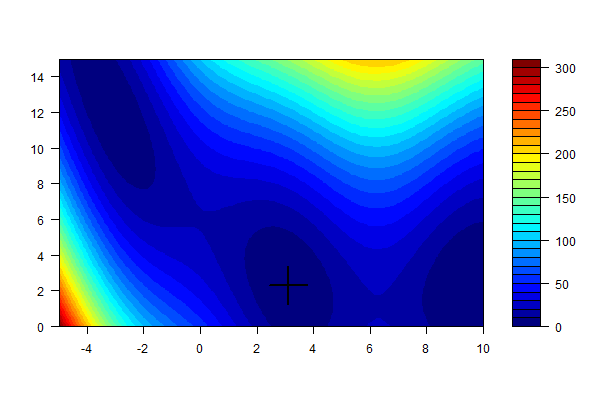
\includegraphics[width=0.7\textwidth]{./assets/Branin6elt.png}
	\caption{Poglądowa lokalizacja najlepszego znalezionego minimum funkcji Branin dla pomiarów przy zmianach elityzmu}
	\label{fig:branin6elt}
\end{figure}

\newpage
\subsection{Gulf (3 parametry)}
\paragraph{}
Gulf jest funkcją określoną dla ilości parametrów równej 3. Na ilustracji (rys.~\ref{fig:gulf1}) przedstawiono jej wykres dla pierwszych dwóch.

\begin{equation}\label{eq:gulf}
f(\boldsymbol{x}) = \sum_{i=1}^{99} [\exp(- \frac{(u_i - x_2)^{x_3}}{x_1}) - 0.01i]^2
\end{equation}

, gdzie $ x_1 \in [0.1, 100] $, $ x_2 \in [0, 25.6] $, $ x_3 \in [0, 5] $ oraz $ u_i = 25 + [-50 \ln (0.01i)]^{1/1.5} $.

\begin{figure}[H]
	\begin{center}
		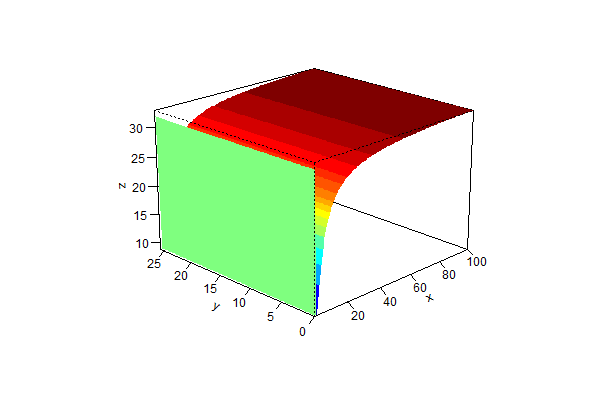
\includegraphics[width=0.95\textwidth]{./assets/Gulf1.png}
		\caption{Wykres funkcji Gulf dla dwóch pierwszych parametrów}
		\label{fig:gulf1}
	\end{center}
\end{figure}

\fbi
Wykres ten przedstawia trójwymiarowy obraz funkcji Gulf dla trzech parametrów, na którym można zauważyć wzrost wartości wraz ze wzrostem osi x.

\fbi
Na kolejnych stronach zamieszczono wyniki pomiarów dla różnych wartości parametrów algorytmu genetycznego.

\begin{figure}[H]
	\begin{center}
		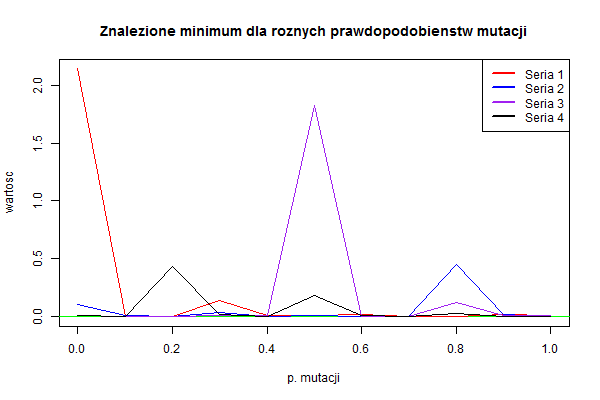
\includegraphics[width=0.85\textwidth]{./assets/Gulf2.png}
		\caption{Wartość znalezionego minimum dla funkcji Gulf w~zależności od prawdopodobieństwa mutacji}
		\label{fig:gulf2}
	\end{center}
\end{figure}

\begin{figure}[H]
	\begin{center}
		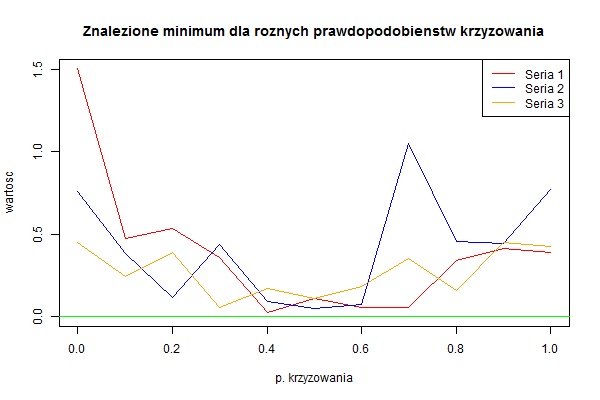
\includegraphics[width=0.85\textwidth]{./assets/Gulf3.png}
		\caption{Wartość znalezionego minimum dla funkcji Gulf w~zależności od prawdopodobieństwa krzyżowania}
		\label{fig:gulf3}
	\end{center}
\end{figure}

\fbi
Wartości funkcji Gulf dla zadanego prawdopodobieństwa mutacji(rys.~\ref{fig:gulf2}) pokazują nikły wpływ na wartość otrzymanych wyników. Wszystkie wartości utrzymują się na poziomie zbliżonym do optimum, wyjątkiem są skoki niektórych wyników, za co odpowiada heurestyka algorytmu genetycznego.

\fbi
Prawdopodobieństwo krzyżowania(rys.~\ref{fig:gulf3}) ma widoczny wpływ na otrzymane wyniki. Wraz ze zwiększeniem wartości krzyżowania rezultat był coraz lepszy. Od przyjętej wartości równej 0,5 wyniki zbliżyły się do optimum funkcji.

\begin{figure}[H]
	\begin{center}
		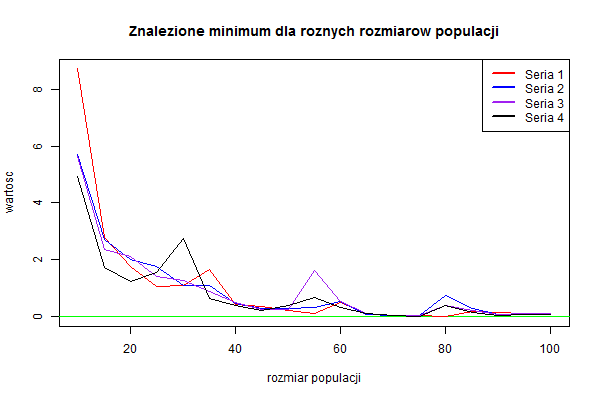
\includegraphics[width=0.85\textwidth]{./assets/Gulf4.png}
		\caption{Wartość znalezionego minimum dla funkcji Gulf w~zależności od rozmiarów populacji}
		\label{fig:gulf4}
	\end{center}
\end{figure}

\begin{figure}[H]
	\begin{center}
		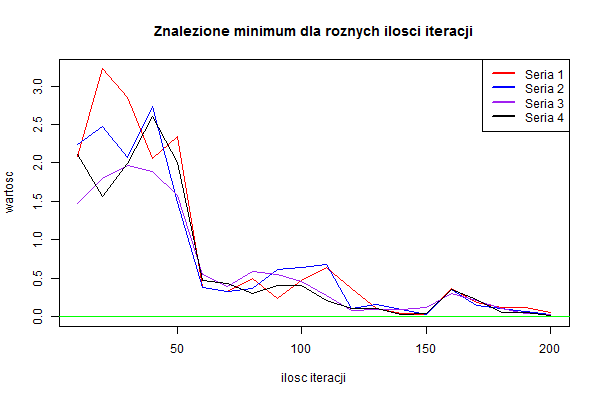
\includegraphics[width=0.85\textwidth]{./assets/Gulf5.png} 
		\caption{Wartość znalezionego minimum dla funkcji Gulf w~zależności od ilości iteracji}
		\label{fig:gulf5}
	\end{center}
\end{figure}

\fbi
Wykres(rys.~\ref{fig:gulf4}) znalezionego minimum dla rozmiarów populacji wyraźnie obrazuje pozytywny wpływ zwiększenia populacji na jakość wyników. Najlepsze wyniki uzyskano dla populacji wynoszącej przynajmniej 40 jednostek.

\fbi
Na wykresie(rys.~\ref{fig:gulf5}) można zauważyć znaczące poprawienie się rezultatów, gdy ilość iteracji wynosi przynamniej 60. Poniżej tej wartości uzyskane wyniki są znacząco gorsze od optymalnego rozwiązania. 

\begin{figure}[H]
	\begin{center}
		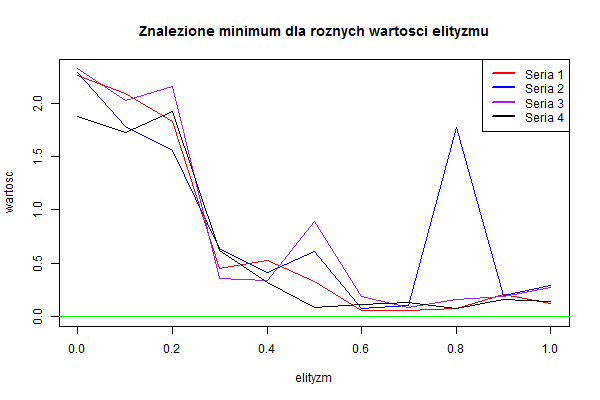
\includegraphics[width=0.85\textwidth]{./assets/Gulf6.png}
		\caption{Wartość znalezionego minimum dla funkcji Gulf w~zależności od przyjętego elityzmu}
		\label{fig:gulf6}
	\end{center}
\end{figure}

\fbi
W przypadku funkcji Gulf elityzm ma znaczący wpływ na otrzymywane wyniki. W celu ich optymalizacji wymagana jest wartość elityzmu na poziomie przynajmniej 0,3.

\newpage
\subsection{CosMix4 (4 parametry)}
\paragraph{}
CosMix4 jest funkcją określoną dla ilości parametrów równej 4. Na ilustracji (rys.~\ref{fig:cosmix41}) przedstawiono jej wykres dla pierwszych dwóch.

\begin{equation}\label{eq:cosmix4}
f(\boldsymbol{x}) = -0.1 \sum_{i=1}^{4} \cos (5 \pi x_i) - \sum_{i=1}^{4} x_i^2
\end{equation}

, gdzie $ x_i \in [-2, 1] $ oraz $ i~= \{1, ... ,4\} $.

\begin{figure}[H]
	\begin{center}
		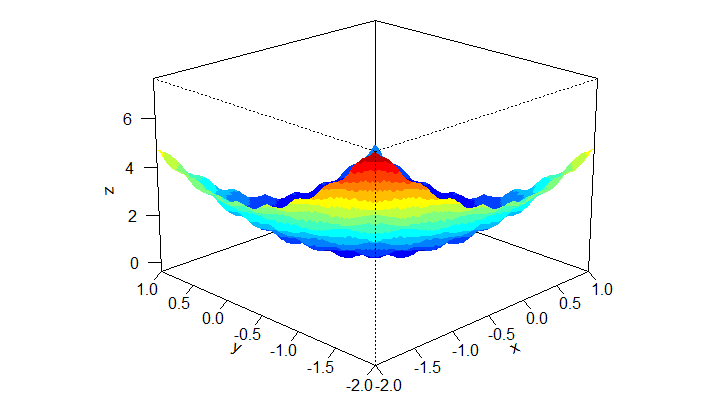
\includegraphics[width=0.95\textwidth]{./assets/CosMix41.png}
		\caption{Wykres funkcji CosMix4 dla dwóch pierwszych parametrów}
		\label{fig:cosmix41}
	\end{center}
\end{figure}

\fbi
Ilustracja powyżej (rys.~\ref{fig:cosmix41}) przedstawia wykres dwóch pierwszych wymiarów dla czterowymiarowej funkcji Cosinus Mixture. 

\begin{figure}[H]
	\begin{center}
		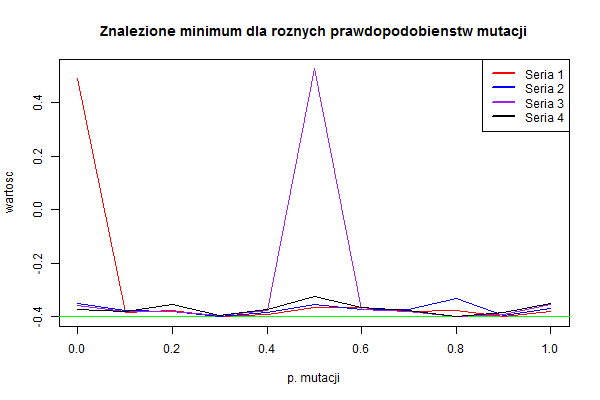
\includegraphics[width=0.85\textwidth]{./assets/CosMix42.png}
		\caption{Wartość znalezionego minimum dla funkcji CosMix4 w~zależności od prawdopodobieństwa mutacji}
		\label{fig:cosmix42}
	\end{center}
\end{figure}

\begin{figure}[H]
	\begin{center}
		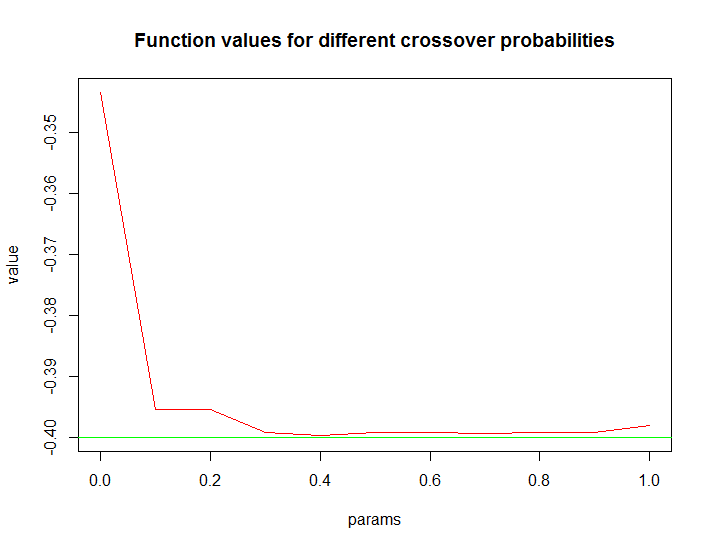
\includegraphics[width=0.85\textwidth]{./assets/CosMix43.png}
		\caption{Wartość znalezionego minimum dla funkcji CosMix4 w~zależności od prawdopodobieństwa krzyżowania}
		\label{fig:cosmix43}
	\end{center}
\end{figure}

\fbi
Z wykresu(rys.~\ref{fig:cosmix42}) wynika nikły wpływ mutacji na otrzymane wyniki. Wartości utrzymują sie w~pobliżu optimum.

\fbi
Wartość krzyżowania powoduje niestabilność wyników w~przedziale (0,0~--~0.6)(rys.~\ref{fig:cosmix44}), dalej wartości osiągają optimum. Wyjątkiem jest wartość 0,8, w~której widoczne jest obniżenie jakości otrzymanych wyników.


\begin{figure}[H]
	\begin{center}
		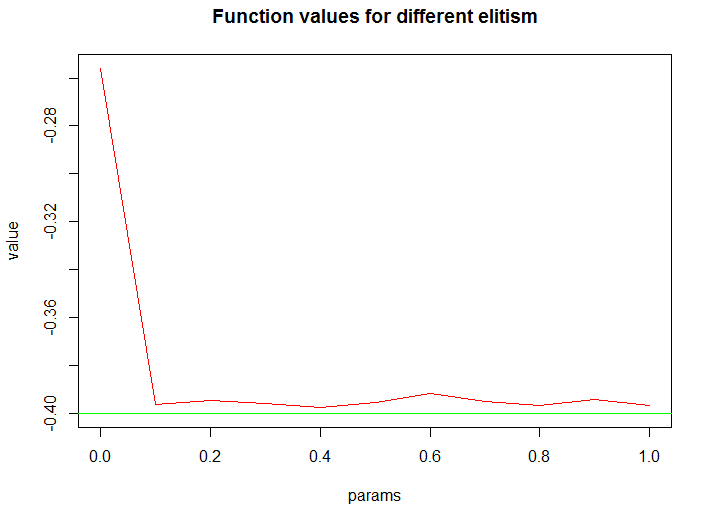
\includegraphics[width=0.85\textwidth]{./assets/CosMix44.png}
		\caption{Wartość znalezionego minimum dla funkcji CosMix4 w~zależności od rozmiarów populacji}
		\label{fig:cosmix44}
	\end{center}
\end{figure}

\begin{figure}[H]
	\begin{center}
		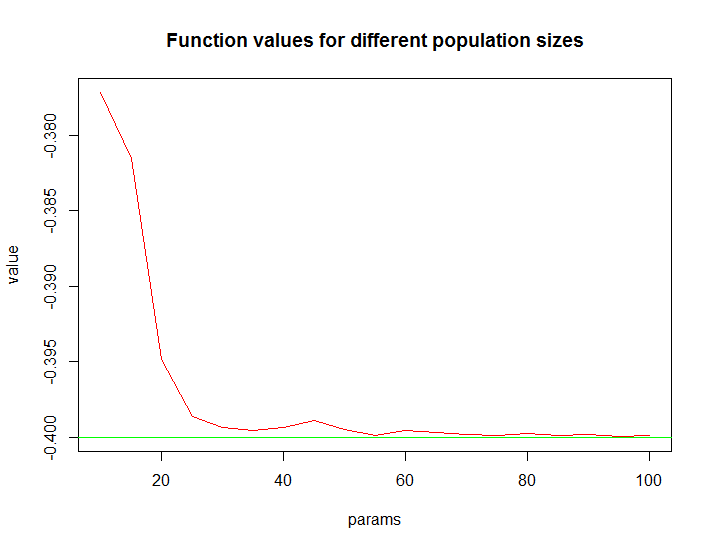
\includegraphics[width=0.85\textwidth]{./assets/CosMix45.png}
		\caption{Wartość znalezionego minimum dla funkcji CosMix4 w~zależności od ilości iteracji}
		\label{fig:cosmix45}
	\end{center}
\end{figure}

\fbi
Na dwóch poprzedzających wykresach(rys.~\ref{fig:cosmix44},\ref{fig:cosmix45}) możemy zaobserwować, że domyślne wartości w~postaci wielkości populacji w~liczbie 40 i~ilości iteracji równej 60 są wzajemnie optymalne.

\fbi
Funkcja osiąga optimum dla wartości populacji równej 85, oraz 170 ilości iteracji.

\fbi
Zauważalne są tutaj pogroszenia się wyników dla wszystkich serii, gdy ilość iteracji wynosi 110. Wynikać to może z~budowy funkcji, która dla tych parametrów zwraca gorsze wyniki.

\begin{figure}[H]
	\begin{center}
		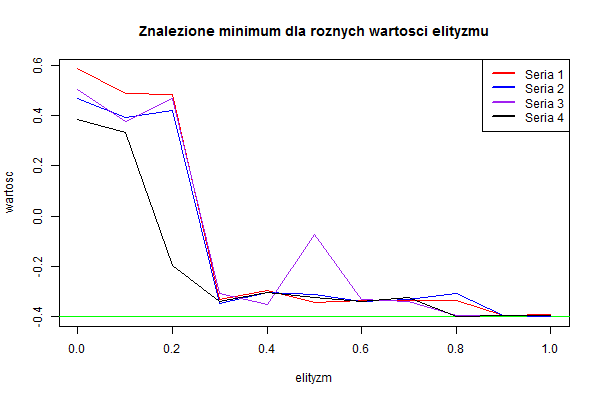
\includegraphics[width=0.85\textwidth]{./assets/CosMix46.png}
		\caption{Wartość znalezionego minimum dla funkcji CosMix4 w~zależności od przyjętego elityzmu}
		\label{fig:cosmix46}
	\end{center}
\end{figure}

\newpage
\subsection{EMichalewicz (5 parametrów)}
\paragraph{}
Poniżej zamieszczono wzór rozpatrywanej funkcji.

\begin{equation}\label{eq:emichalewicz}
f(\boldsymbol{x}) = - \sum_{i=1}^{d} \sin(x_i) \sin^{2m} (\frac{i x_i^2}{\pi})
\end{equation}

, gdzie $ x_i \in [0, \pi]$ oraz $j = \{1, ..., 5\}$.

\begin{figure}[H]
	\begin{center}
		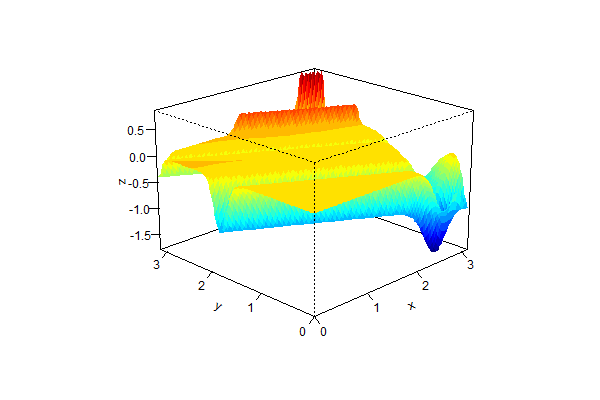
\includegraphics[width=0.95\textwidth]{./assets/EMichalewicz1.png}
		\caption{Wykres funkcji EMichalewicz dla dwóch pierwszych wymiarów}
		\label{fig:emichalewicz1}
	\end{center}
\end{figure}

\begin{figure}[H]
	\begin{center}
		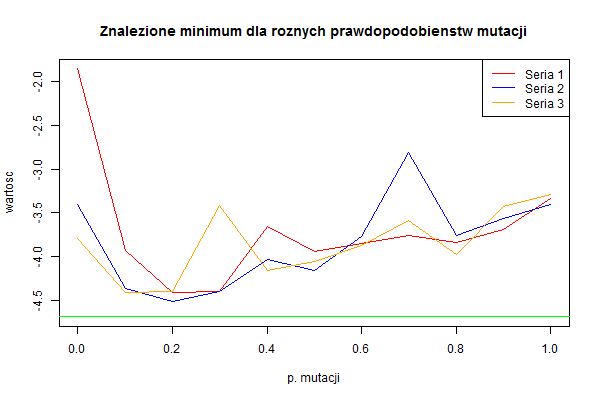
\includegraphics[width=0.85\textwidth]{./assets/EMichalewicz2.png}
		\caption{Wartość znalezionego minimum dla funkcji EMichalewicz w~zależności od prawdopodobieństwa mutacji}
		\label{fig:emichalewicz2}
	\end{center}
\end{figure}

\begin{figure}[H]
	\begin{center}
		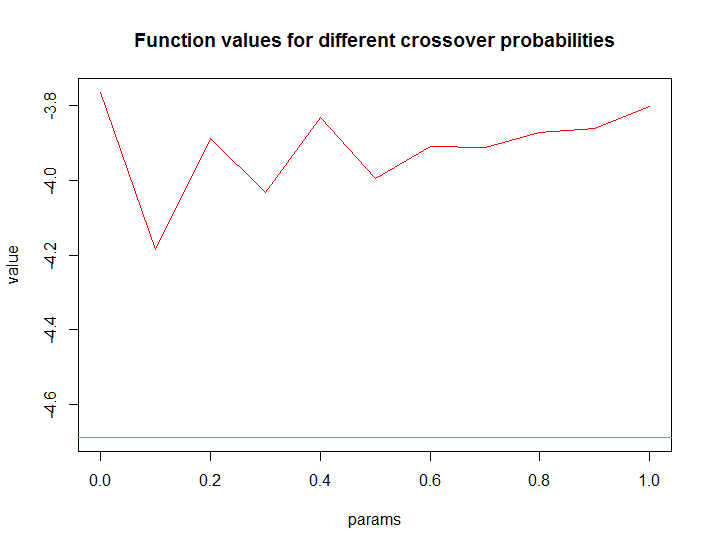
\includegraphics[width=0.85\textwidth]{./assets/EMichalewicz3.png}
		\caption{Wartość znalezionego minimum dla funkcji EMichalewicz w~zależności od prawdopodobieństwa krzyżowania}
		\label{fig:emichalewicz3}
	\end{center}
\end{figure}

\fbi
Oba wykresy (~rys.\ref{fig:emichalewicz1},\ref{fig:emichalewicz2}) pokazują minimalny wpływ prawdopodobieństwa krzyżowania oraz mutacji na wpływ otrzymywanych wyników. 

\fbi
Z wykonanych pomiarów nie można odczytać dla jakich wartości mutacji, czy krzyżowania funkcja zbliża się od optimum. Najblżej optimum była mutacja na dowolnym, niezerowym poziomie.

\begin{figure}[H]
	\begin{center}
		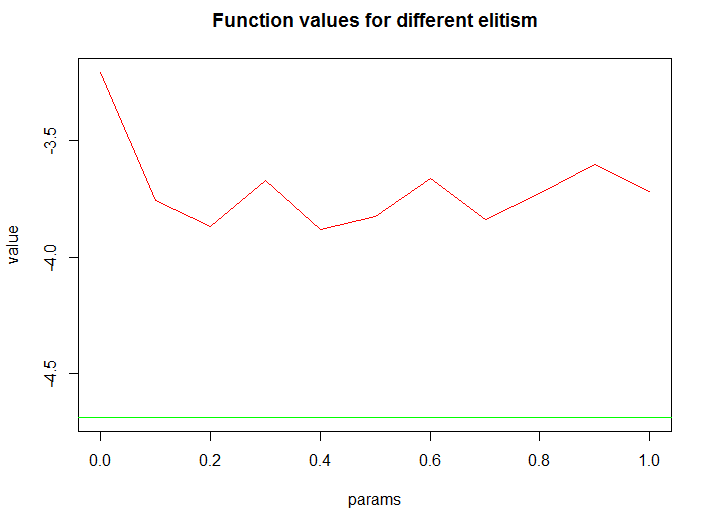
\includegraphics[width=0.85\textwidth]{./assets/EMichalewicz4.png}
		\caption{Wartość znalezionego minimum dla funkcji EMichalewicz w~zależności od rozmiarów populacji}
		\label{fig:emichalewicz4}
	\end{center}
\end{figure}


\begin{figure}[H]
	\begin{center}
		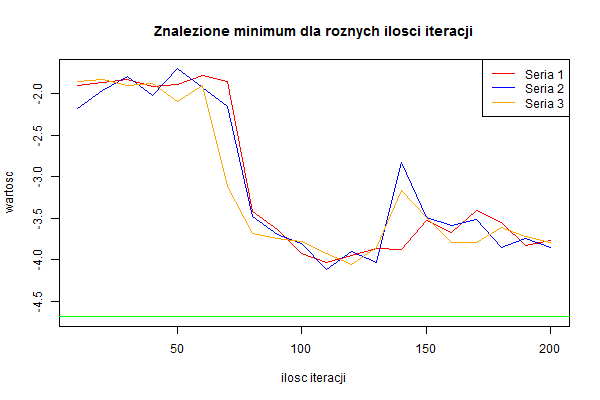
\includegraphics[width=0.85\textwidth]{./assets/EMichalewicz5.png}
		\caption{Wartość znalezionego minimum dla funkcji EMichalewicz w~zależności od ilości iteracji}
		\label{fig:emichalewicz5}
	\end{center}
\end{figure}

\fbi
Z wykresu(\ref{fig:emichalewicz3}) można odczytać wpływ zwiększenia populacji na jakość otrzymywanych wyników. Funkcja ta logarytmicznie dąży do pewnej wartości, lecz nie jest to wartość optimum. Oznacza to, że modyfikacja samej tylko populacji nie osiągnie optimum dla danej funkcji.

\fbi
Ilość iteracji ma znaczący wpływ na otrzymane wyniki od wartości równej 50. W dalszym etapie funkcja zbliża się do optimum.

\begin{figure}[H]
	\begin{center}
		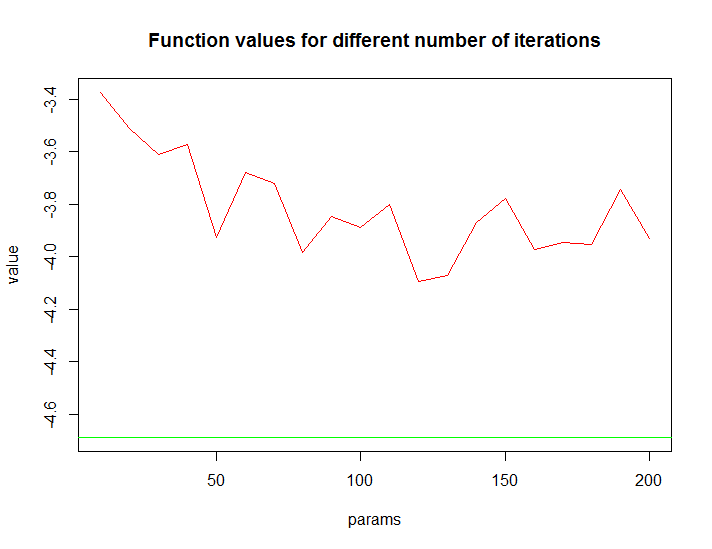
\includegraphics[width=0.85\textwidth]{./assets/EMichalewicz6.png}
		\caption{Wartość znalezionego minimum dla funkcji EMichalewicz w~zależności od przyjętego elityzmu}
		\label{fig:emichalewicz6}
	\end{center}
\end{figure}

\fbi
Tak samo jak w~przypadku wykresu populacji(\ref{fig:emichalewicz3}) elityzm logartymicznie dąży do pewniej wartości, lecz nie do optimum funkcji. Zwiększenie ilości elit w~populacji w~przypadku funkcji EMichalewicza poprawia jakość otrzymywanych wyników.

\fbi
Wybranie elityzmu na poziomie niższym niż 0,2 powoduje otrzymywanie około dwuktrotnie gorszych wyników niż otrzymano na dowolnie innym poziomie.

\newpage
\subsection{Hartman6 (6 parametrów)}
\paragraph{}
Hartman6 jest funkcją określoną dla ilości parametrów równej 6. Na ilustracji (rys.~\ref{fig:hartman61}) przedstawiono jej wykres dla pierwszych dwóch.

\begin{equation}\label{eq:hartman6}
f(\boldsymbol{x}) = - \sum_{i=1}^{4} c_i \exp[- \sum_{j=1}^{6} a_{ij}(x_j - p_{ij})^2]
\end{equation}

, gdzie $ x_i \in [0, 1] $, $ i~\in \{1, ..., 6\} $.

\begin{figure}[H]
	\begin{center}
		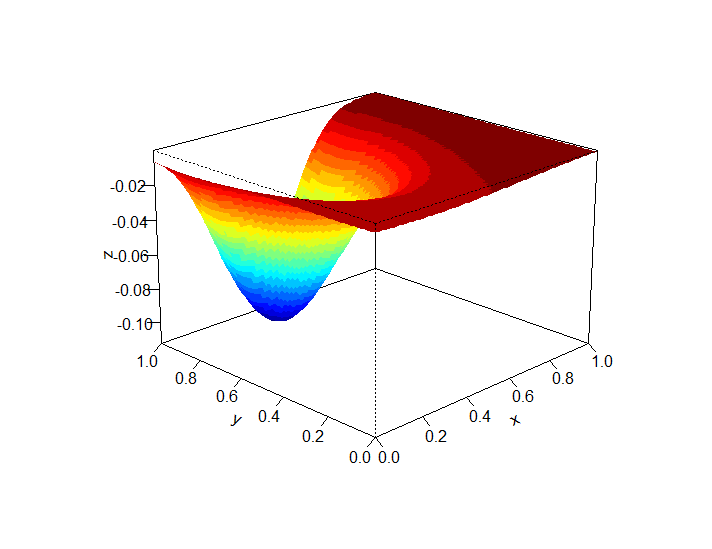
\includegraphics[width=0.95\textwidth]{./assets/Hartman61.png}
		\caption{Wykres funkcji Hartman6 dla dwóch pierwszych parametrów}
		\label{fig:hartman61}
	\end{center}
\end{figure}

\begin{figure}[H]
	\begin{center}
		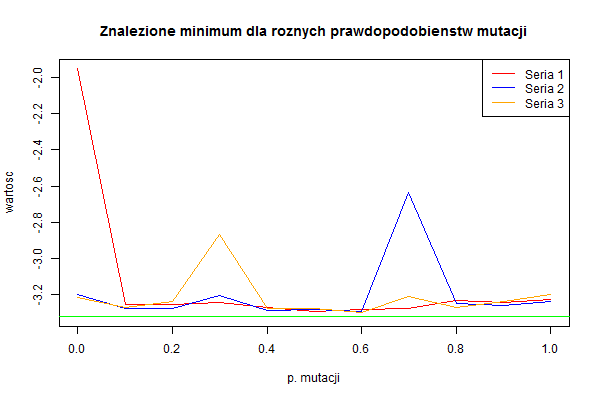
\includegraphics[width=0.85\textwidth]{./assets/Hartman62.png}
		\caption{Wartość znalezionego minimum dla funkcji Hartman6 w~zależności od prawdopodobieństwa mutacji}
		\label{fig:hartman62}
	\end{center}
\end{figure}

\begin{figure}[H]
	\begin{center}
		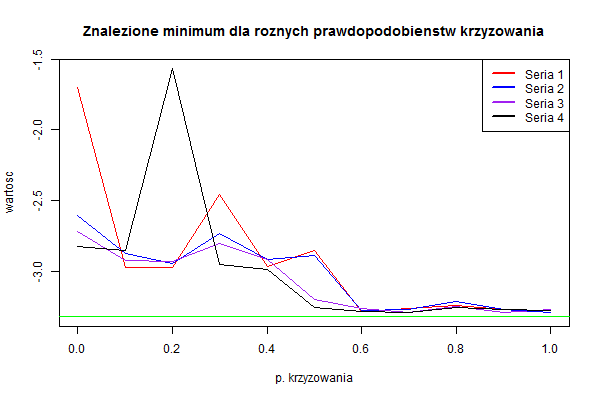
\includegraphics[width=0.85\textwidth]{./assets/Hartman63.png}
		\caption{Wartość znalezionego minimum dla funkcji Hartman6 w~zależności od prawdopodobieństwa krzyżowania}
		\label{fig:hartman63}
	\end{center}
\end{figure}

\fbi
Z wykresu(rys.~\ref{fig:hartman61}) odczytać można niski wpływ mutacji na osiągane wyniki. Dla wszystkich wartości mutacji otrzymywane wyniki zbliżone są do optimum funkcji.

\fbi
Warto zauważyć, że wszystkie serie posiadają jedną wartość mutacji, dla której następuje pogorszenie otrzymanego wyniku. Serie posiadają inne wartości domyślne dla funkcji. Oznacza to, że funkcja dla pewnej wartości, określonej przez wartości domyślne, zwraca gorsze wyniki.

\fbi
Wykres krzyżowania(rys.~\ref{fig:hartman62}) wskazuje wartość 0,6 jako graniczną dla otrzymywania optimum funkcji. Przed tą wartością otrzymane wyniki są niestabilne, nie można odczytać nich czy wyniki się poprawiają czy pogarszają.

\begin{figure}[H]
	\begin{center}
		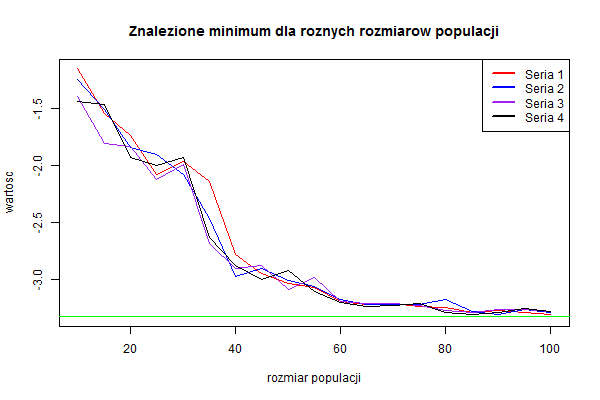
\includegraphics[width=0.85\textwidth]{./assets/Hartman64.png}
		\caption{Wartość znalezionego minimum dla funkcji Hartman6 w~zależności od rozmiarów populacji}
		\label{fig:hartman64}
	\end{center}
\end{figure}


\begin{figure}[H]
	\begin{center}
		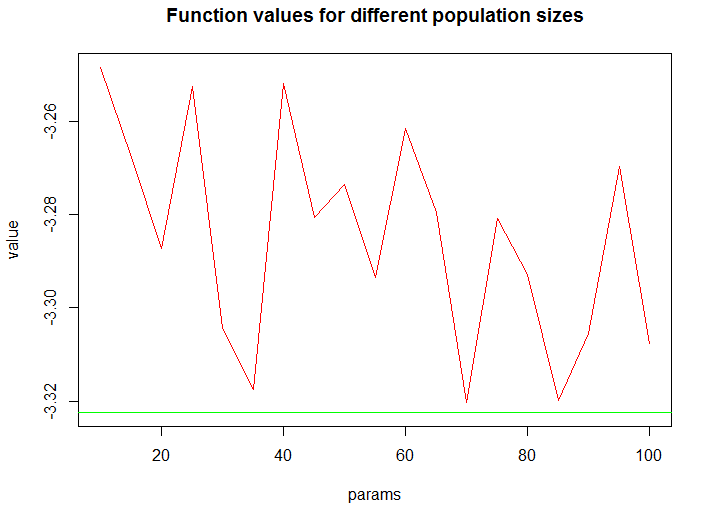
\includegraphics[width=0.85\textwidth]{./assets/Hartman65.png}
		\caption{Wartość znalezionego minimum dla funkcji Hartman6 w~zależności od ilości iteracji}
		\label{fig:hartman65}
	\end{center}
\end{figure}

\fbi
Wykres populacji(rys.~\ref{fig:hartman63}) wskazuje na logarytmiczną zbieżność wartości dla danej populacji do optimum funkcji. Wynika z~tego, że funkcja ta osiąga optimum dla dowolnych parametrów mutacji i~krzyżowania, lecz dużej populacji.

\fbi
Ilość iteracji dąży do optimum dla więcej niż 50 iteracji. Wartość ta jest wartością graniczną. Wyniki znajdujące się przed nią są ponad dwuktornie gorsze niż wyniki po niej. Zauważalne są również dwa skoki (dla wartości 110 i~160) pokazujące pogorszenie rezultatu, wskazują one na budowę funkcji, która dla tych wartości zwraca gorsze wyniki.

\begin{figure}[H]
	\begin{center}
		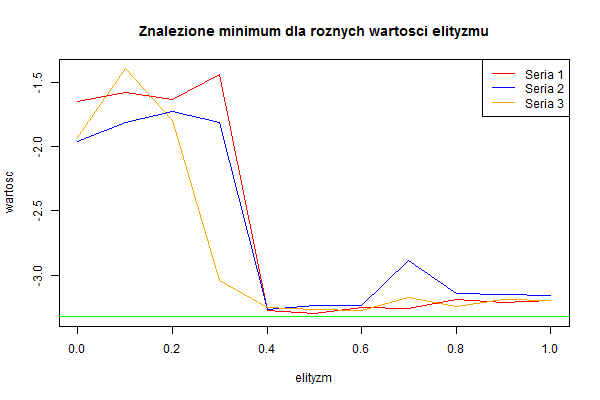
\includegraphics[width=0.85\textwidth]{./assets/Hartman66.png}
		\caption{Wartość znalezionego minimum dla funkcji Hartman6 w~zależności od przyjętego elityzmu}
		\label{fig:hartman66}
	\end{center}
\end{figure}

\fbi
Zwiększenie elityzmu logartymicznie dąży do wartości optymalnej. Wartości, które zostały w~ten sposób osiągnięte, są bliskie optimum, lecz jego nie osiągają. Oznacza to, że samym elityzmem nie można dla danej funkcji osiągnąć wartości optymalnej, a~tylko się do niej zbliżyć.

\newpage
\subsection{PriceTransistor (9 parametrów)}
\paragraph{}
PriceTransistor jest funkcją określoną dla ilości parametrów równej 9. Na ilustracji (rys.~\ref{fig:pricetransistor1}) przedstawiono jej wykres dla pierwszych dwóch.

\begin{equation}\label{eq:pricetransistor}
f(\boldsymbol{x}) = \gamma^2 + \sum_{k=1}^{4} ( \alpha_k^2 + \beta_k^2 )
\end{equation}

, gdzie $ \alpha_k = (1-x_1 x_2)x_3 {\exp[ x^5 (g_{1k} - g_{3k})]}$ oraz $ x_i \in [0, 10]$ dla $i = \{1, ..., 9\}$.

\begin{figure}[H]
	\begin{center}
		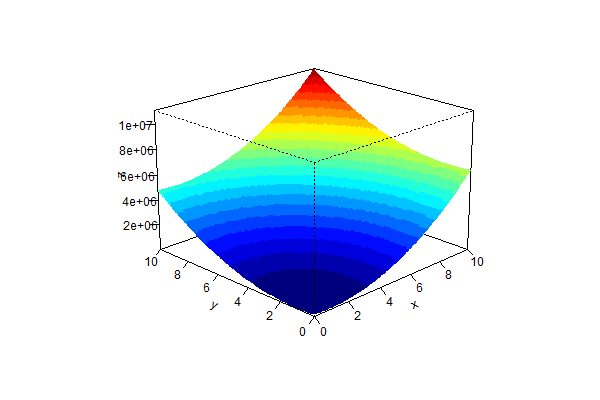
\includegraphics[width=0.95\textwidth]{./assets/PriceTransistor1.png}
		\caption{Wykres funkcji PriceTransistor dla dwóch pierwszych wymiarów}
		\label{fig:pricetransistor1}
	\end{center}
\end{figure}

\begin{figure}[H]
	\begin{center}
		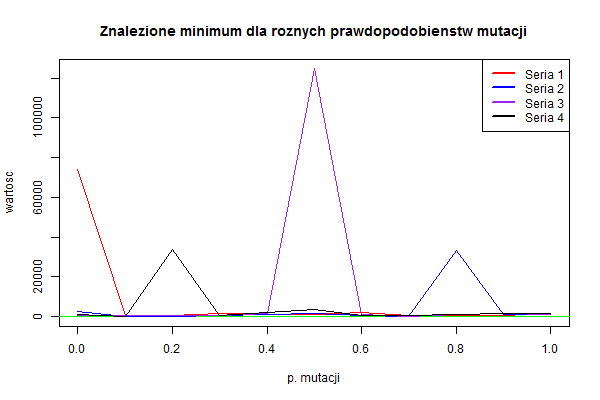
\includegraphics[width=0.85\textwidth]{./assets/PriceTransistor2.png}
		\caption{Wartość znalezionego minimum dla funkcji PriceTransistor w~zależności od prawdopodobieństwa mutacji}
		\label{fig:pricetransistor2}
	\end{center}
\end{figure}

\begin{figure}[H]
	\begin{center}
		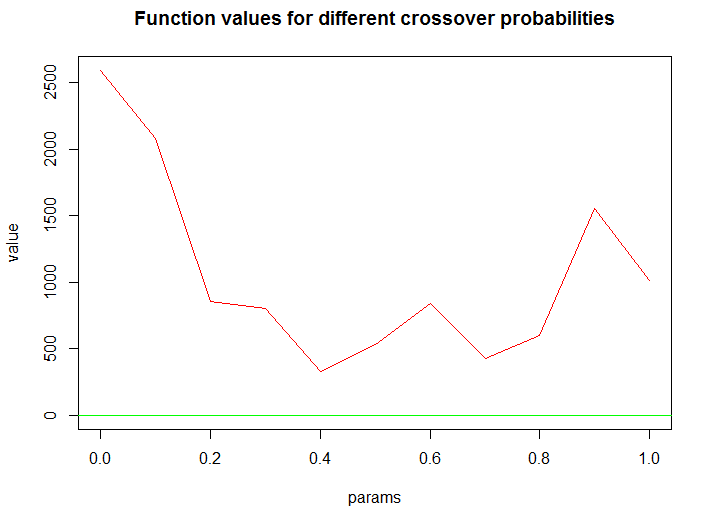
\includegraphics[width=0.85\textwidth]{./assets/PriceTransistor3.png}
		\caption{Wartość znalezionego minimum dla funkcji PriceTransistor w~zależności od prawdopodobieństwa krzyżowania}
		\label{fig:pricetransistor3}
	\end{center}
\end{figure}

\fbi
Na podstawie powyższych wykresów mutacji (rys.~\ref{fig:pricetransistor2}) oraz krzyżowania (rys.~\ref{fig:pricetransistor3}) możemy uznać, że: w~przypadku mutacji wystąpił nieoczekiwany wynik dla wartości 0,5 który ,,spłaszczył'' resztę wykresu, w~przypadku krzyżowania najlepsze wyniki uzyskano dla wartości prawdopodobieństwa powyżej 0,6.

\begin{figure}[H]
	\begin{center}
		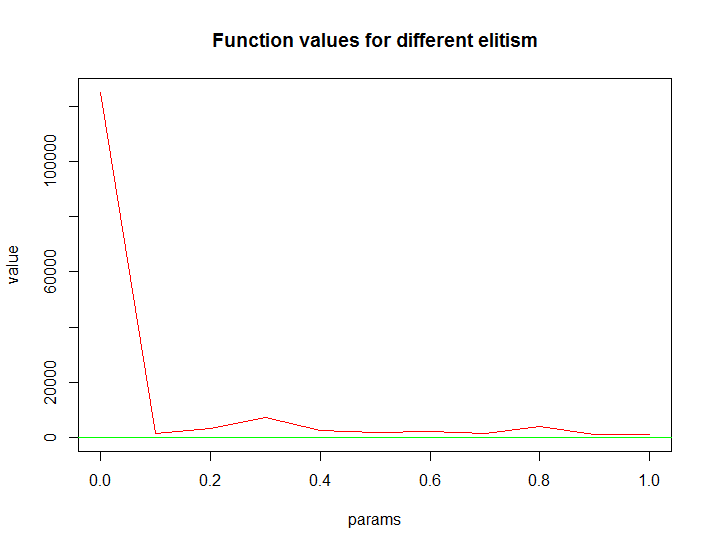
\includegraphics[width=0.85\textwidth]{./assets/PriceTransistor4.png}
		\caption{Wartość znalezionego minimum dla funkcji PriceTransistor w~zależności od rozmiarów populacji}
		\label{fig:pricetransistor4}
	\end{center}
\end{figure}

\begin{figure}[H]
	\begin{center}
		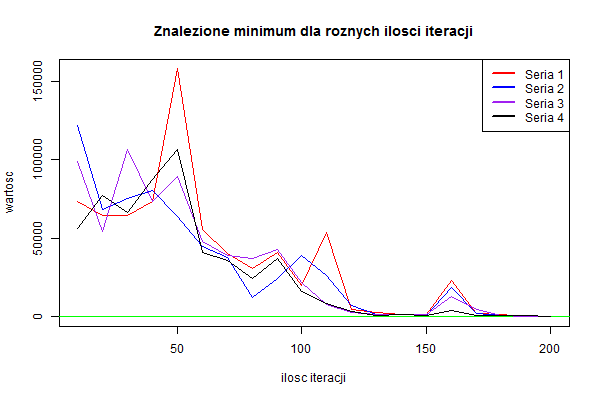
\includegraphics[width=0.85\textwidth]{./assets/PriceTransistor5.png}
		\caption{Wartość znalezionego minimum dla funkcji PriceTransistor w~zależności od ilości iteracji}
		\label{fig:pricetransistor5}
	\end{center}
\end{figure}

\fbi
Na podstawie powyższych wykresów populacji (rys.~\ref{fig:pricetransistor4}) oraz iteracji (rys.~\ref{fig:pricetransistor5}) można zauważyć iż wraz ze wzrostem każdego z~parametrów wyniki ulegają poprawie.

\begin{figure}[H]
	\begin{center}
		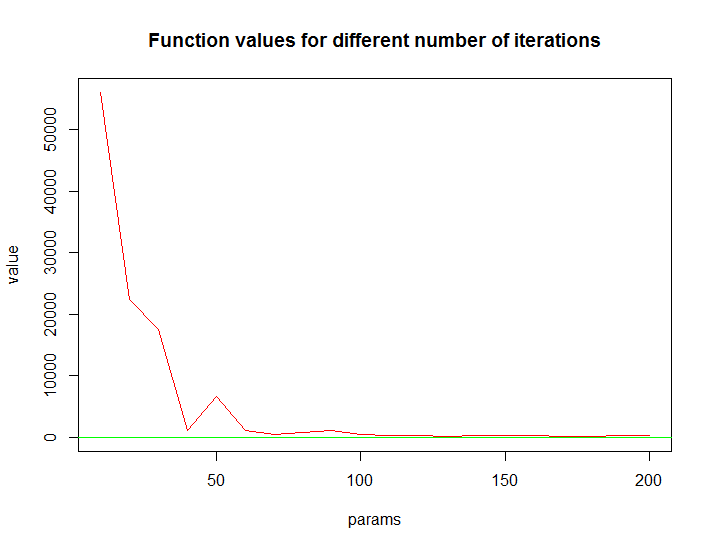
\includegraphics[width=0.85\textwidth]{./assets/PriceTransistor6.png}
		\caption{Wartość znalezionego minimum dla funkcji PriceTransistor w~zależności od przyjętego elityzmu}
		\label{fig:pricetransistor6}
	\end{center}
\end{figure}

\fbi
W przypadku rozpatrywanej funkcji widać (rys.~\ref{fig:pricetransistor6}), że jeden z~wynik dla jednej z~konfiguracji ,,zaburzył'' skalę wykresu.

\newpage
\subsection{Schwefel (10 parametrów)}
\paragraph{}
Schwefel jest funkcją określoną dla ilości parametrów równej 10. Na ilustracji (rys.~\ref{fig:schwefel1}) przedstawiono jej wykres dla pierwszych dwóch.

\begin{equation}\label{eq:schwefel}
f(\boldsymbol{x}) = 418.9829d - \sum_{i=1}^{d} x_i \sin(\sqrt{|x_i|})
\end{equation}

, gdzie $ x_i \in [-500, 500]$ oraz $j = \{1, ..., 10\}$.

\begin{figure}[H]
	\begin{center}
		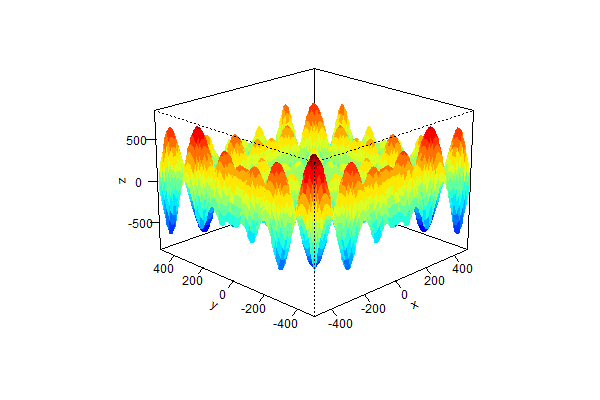
\includegraphics[width=0.95\textwidth]{./assets/Schwefel1.png}
		\caption{Wykres funkcji Schwefel dla dwóch pierwszych wymiarów}
		\label{fig:schwefel1}
	\end{center}
\end{figure}

\fbi
Funkcja ma wiele lokalnych optimów przy domyślnych ograniczeniach (rys.~\ref{fig:schwefel1}) w~związku z~czym możemy ją uznać za trudną w~optymalizacji. 

\begin{figure}[H]
	\begin{center}
		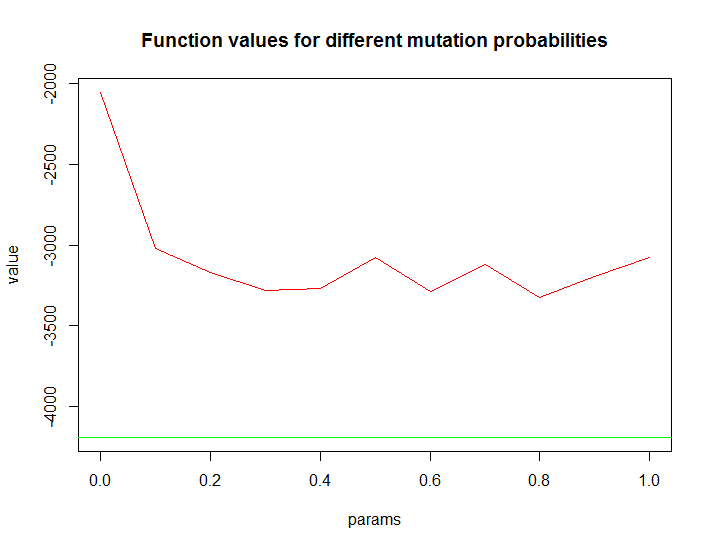
\includegraphics[width=0.85\textwidth]{./assets/Schwefel2.png}
		\caption{Wartość znalezionego minimum dla funkcji Schwefel w~zależności od prawdopodobieństwa mutacji}
		\label{fig:schwefel2}
	\end{center}
\end{figure}

\begin{figure}[H]
	\begin{center}
		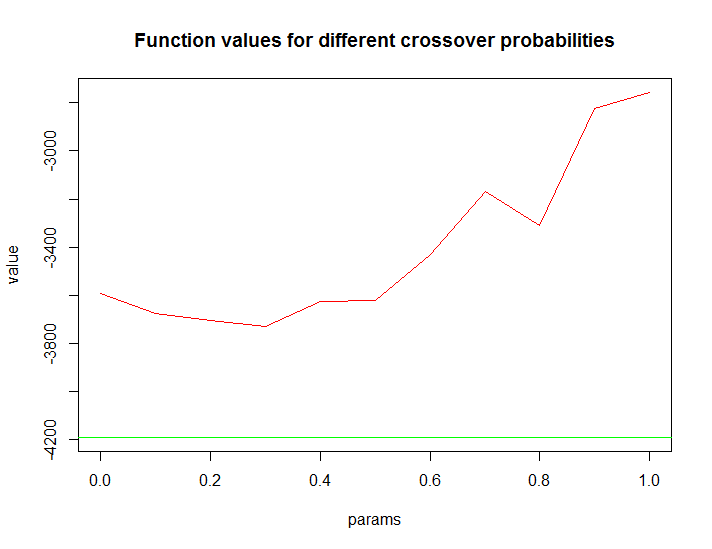
\includegraphics[width=0.85\textwidth]{./assets/Schwefel3.png}
		\caption{Wartość znalezionego minimum dla funkcji Schwefel w~zależności od prawdopodobieństwa krzyżowania}
		\label{fig:schwefel3}
	\end{center}
\end{figure}

\fbi
Na podstawie powyższych wykresów mutacji (rys.~\ref{fig:schwefel2}) oraz krzyżowania (rys.~\ref{fig:schwefel3}) możemy uznać, że relatywnie najlepsze wyniki uzyskujemy dla p. mutacji rzędu 0,6 -- 0,7 oraz p. krzyżowania rzędu 0,6 lub 0,9.

\begin{figure}[H]
	\begin{center}
		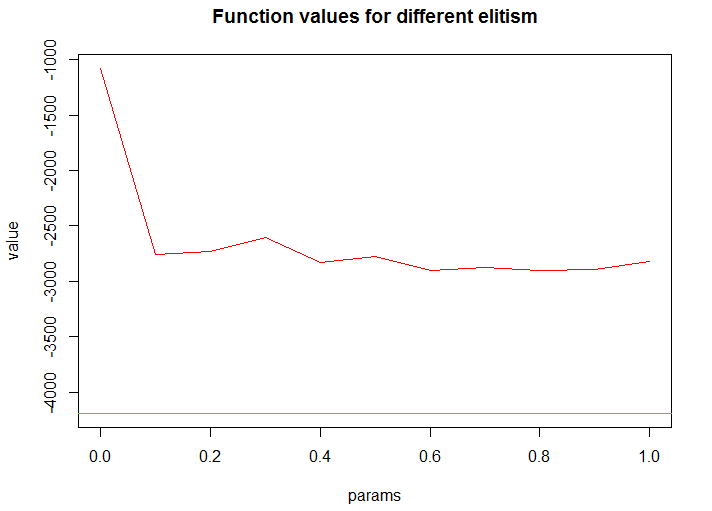
\includegraphics[width=0.85\textwidth]{./assets/Schwefel4.png}
		\caption{Wartość znalezionego minimum dla funkcji Schwefel w~zależności od rozmiarów populacji}
		\label{fig:schwefel4}
	\end{center}
\end{figure}

\begin{figure}[H]
	\begin{center}
		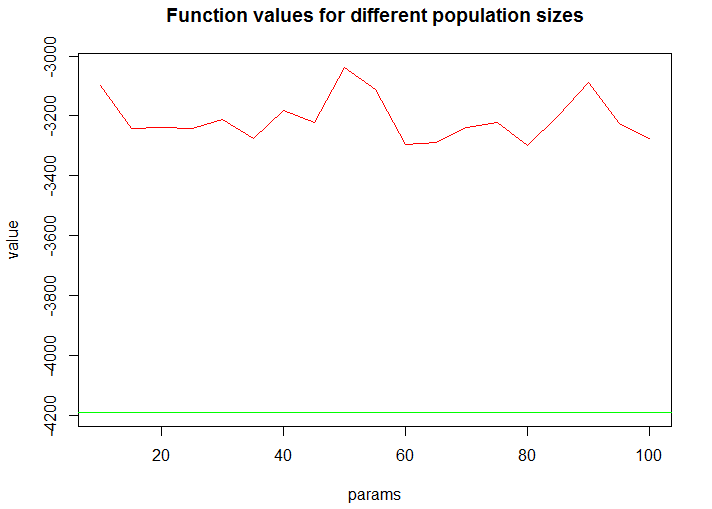
\includegraphics[width=0.85\textwidth]{./assets/Schwefel5.png}
		\caption{Wartość znalezionego minimum dla funkcji Schwefel w~zależności od ilości iteracji}
		\label{fig:schwefel5}
	\end{center}
\end{figure}

\fbi
Na podstawie powyższych wykresów populacji (rys.~\ref{fig:schwefel4}) oraz iteracji (rys.~\ref{fig:schwefel5}) można zauważyć iż zachodzą pewne prawidłowości lecz nie są one całkowicie zgodne z~intuicją jeżeli o~takowej możemy tu mówić. Optymalny rozmiar populacji zdaje się wynosić 75. Natomiast ilość iteracji powyżej 150 chwilowo pogarsza wyniki, jednak jak widać dla większych wartości ponownie się one polepszają. Warto zauważyć, że dla ilości iteracji 150 nie osiągane jest optimum zatem przypuszczalnie wzrost ilości iteracji powinien tu pomóc. Wszystko zależy też od tego ile czasu możemy przeznaczyć na poszukiwania.

\begin{figure}[H]
	\begin{center}
		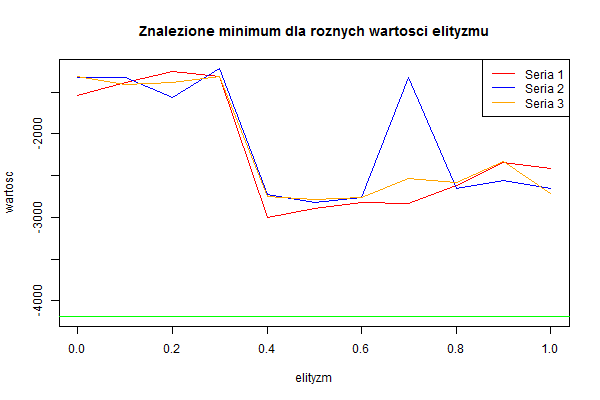
\includegraphics[width=0.85\textwidth]{./assets/Schwefel6.png}
		\caption{Wartość znalezionego minimum dla funkcji Schwefel w~zależności od przyjętego elityzmu}
		\label{fig:schwefel6}
	\end{center}
\end{figure}

\fbi
W przypadku rozpatrywanej funkcji najlepsze rezultaty otrzymano (rys.~\ref{fig:schwefel6}) dla wartości elityzmu rzędu 0,6 -- 0,7. Oznacza to, że gdy trochę więcej niż połowa osobników przechodzi do kolejnego pokolenia uzyskujemy najlepsze wyniki.

\fbi
Analizując otrzymane rezultaty całościowo możemy stwierdzić, że w~żadnym przypadku nie udało się otrzymać wartości optymalnej. Jest to związane ze stosunkowo dużą przestrzenią poszukiwań i~dużą ilością lokalnych optimów.

\newpage
\subsection{Zeldasine20 (20 parametrów)}
\paragraph{}
Zeldasine20 jest funkcją określoną dla ilości parametrów równej 20. Na ilustracji (rys.~\ref{fig:zeldasine1}) przedstawiono jej wykres dla pierwszych dwóch.

\begin{equation}\label{eq:zeldasine}
f(\boldsymbol{x}) = -A \prod_{j=1}^{D} \sin (x_j - z) - \prod_{j=1}^{D} \sin (B \cdot (x_j - z))
\end{equation}

, gdzie $ x_j \in [0, \pi]$ oraz $j = \{1, ..., 20\}$.

\begin{figure}[H]
	\begin{center}
		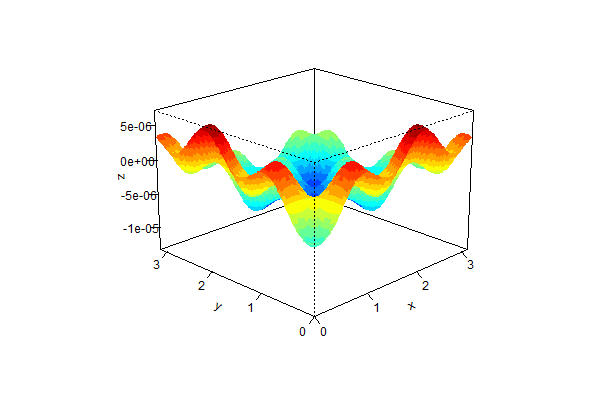
\includegraphics[width=0.95\textwidth]{./assets/Zeldasine201.png}
		\caption{Wykres funkcji Zeldasine20 dla dwóch pierwszych parametrów}
		\label{fig:zeldasine1}
	\end{center}
\end{figure}

\fbi
Funkcja ma bardzo pofalowaną powierzchnię i~dużo lokalnych optimów. Można intuicyjnie założyć, że jest ciężka do optymalizacji.

\begin{figure}[H]
	\begin{center}
		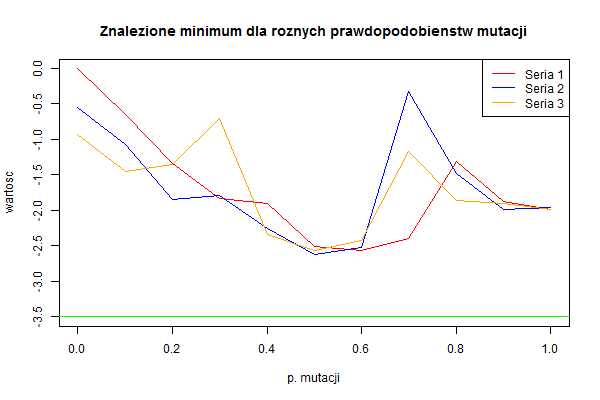
\includegraphics[width=0.85\textwidth]{./assets/Zeldasine202.png}
		\caption{Wartość znalezionego minimum dla funkcji Zeldasine20 w~zależności od prawdopodobieństwa mutacji}
		\label{fig:zeldasine2}
	\end{center}
\end{figure}

\begin{figure}[H]
	\begin{center}
		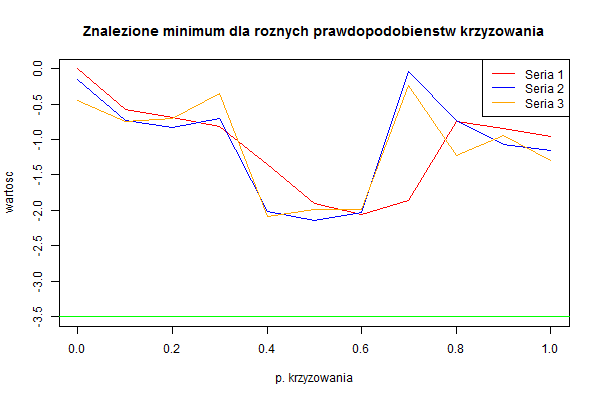
\includegraphics[width=0.85\textwidth]{./assets/Zeldasine203.png}
		\caption{Wartość znalezionego minimum dla funkcji Zeldasine20 w~zależności od prawdopodobieństwa krzyżowania}
		\label{fig:zeldasine3}
	\end{center}
\end{figure}

\fbi
Na podstawie powyższych wykresów mutacji (rys.~\ref{fig:zeldasine2}) oraz krzyżowania (rys.~\ref{fig:zeldasine3}) możemy uznać, że relatywnie najlepsze wyniki uzyskujemy dla p. mutacji rzędu 0,4 oraz p. krzyżowania rzędu 0,6.

\begin{figure}[H]
	\begin{center}
		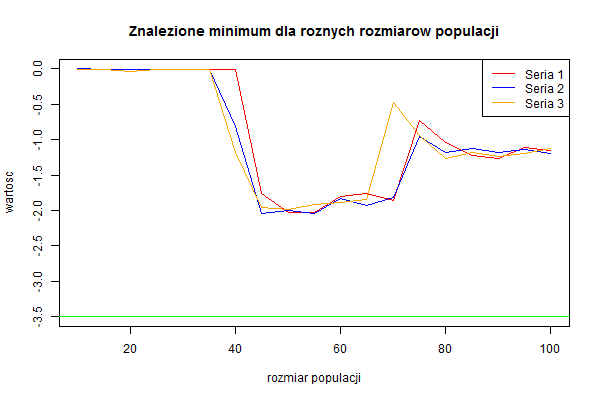
\includegraphics[width=0.85\textwidth]{./assets/Zeldasine204.png}
		\caption{Wartość znalezionego minimum dla funkcji Zeldasine20 w~zależności od rozmiarów populacji}
		\label{fig:zeldasine4}
	\end{center}
\end{figure}

\begin{figure}[H]
	\begin{center}
		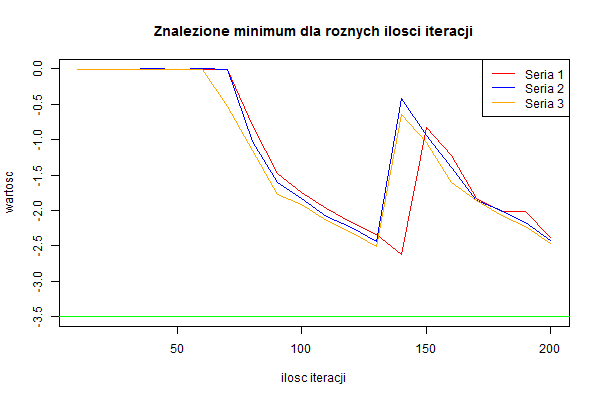
\includegraphics[width=0.85\textwidth]{./assets/Zeldasine205.png}
		\caption{Wartość znalezionego minimum dla funkcji Zeldasine20 w~zależności od ilości iteracji}
		\label{fig:zeldasine5}
	\end{center}
\end{figure}

\fbi
Na podstawie powyższych wykresów populacji (rys.~\ref{fig:zeldasine4}) oraz iteracji (rys.~\ref{fig:zeldasine5}) możemy uznać, że wzrost rozmiaru populacji i~ilości iteracji wpływa pozytywnie na jakość rezultatów. Zwłaszcza zwiększanie ilości iteracji w~przypadku funkcji z~tak dużą ilością parametrów zdaje się prowadzić w~dobrym kierunku.

\begin{figure}[H]
	\begin{center}
		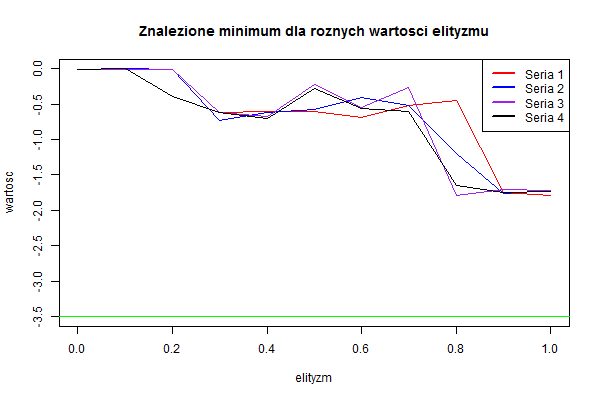
\includegraphics[width=0.85\textwidth]{./assets/Zeldasine206.png}
		\caption{Wartość znalezionego minimum dla funkcji Zeldasine20 w~zależności od przyjętego elityzmu}
		\label{fig:zeldasine6}
	\end{center}
\end{figure}

\fbi
W przypadku rozpatrywanej funkcji najlepsze rezultaty otrzymano (rys.~\ref{fig:zeldasine6}) dla wartości elityzmu rzędu 0,9 -- 1,0. Oznacza to, że gdy wszystkie osobniki przechodzą do kolejnego pokolenia uzyskujemy najlepsze wyniki.

\fbi
Analizując otrzymane rezultaty możemy stwierdzić, że w~żadnym przypadku nie udało się otrzymać wartości bliskiej szukanemu optimum. Jest to związane z~dużą przestrzenią poszukiwań. Musimy pamiętać, że rozpatrujemy tu funkcję o~20 parametrach.

\newpage
\section{Podsumowanie}
\paragraph{}
W trakcie prowadzonych badań przetestowano algorytm genetyczny w~zadaniu optymalizacji dla 9 funkcji testowych. Analizie poddano wpływ zmiany każdego z~parametrów dla 4 różnych konfiguracji pozostałych wartości domyślnych.

\fbi
Wartość prawdopodobieństwa mutacji i~krzyżowania zdaje się odgrywać drugorzędną rolę. Istotne jednak by chociaż jedna z~nich była włączona z~prawdopodobieństwem większym niż 0.

\fbi
Najlepszym ustawieniem dla elityzmu jest prawdopodobieństwo rzędu 0,5.

\fbi
Z pewnością należałoby zwiększyć ilość prób poddawanych uśrednianiu gdyż dla przyjętych 20 wyniki ciągle są niestabilne. Warto by również rozważyć pomijanie kilku najlepszych i~najgorszych wyników przed uśrednianiem.

\fbi
Co ciekawe wyniki są widocznie gorsze przy konfiguracji w~której krzyżowanie jest wyłączone a~p. mutacji wynosi 0,5. Taka prawidłowość objawia się dla wszystkich badanych funkcji.

\newpage
\begin{thebibliography}{40}

\bibitem{test1}
Artur Suchwałko ,,Wprowadzenie do R dla programistów innych języków'' https://cran.r-project.org/doc/contrib/R-dla-programistow-innych-jezykow.pdf

\bibitem{test2}
Luca Scrucca ,,A quick tour of GA''
https://cran.r-project.org/web/packages/GA/vignettes/GA.html

\bibitem{test3}
Surjanovic, S. \& Bingham, D. (2013). ,,Virtual Library of Simulation Experiments: Test Functions and Datasets.'' Retrieved April 3, 2017, from http://www.sfu.ca/~ssurjano.

\bibitem{test4}
Momin Jamil, Xin-She Yang ,,A literature survey of benchmark functions for global optimization problems'', Int. Journal of Mathematical Modelling and Numerical Optimisation, Vol. 4, No. 2, pp. 150–194. (2013)

\bibitem{test5}
Ajith Abraham, Aboul-Ella Hassanien, Patrick Siarry, Andries Engelbrecht, ,,Foundations of Computational Intelligence Volume 3'' (2009)

\bibitem{test6}
Onay Urfalioglu, Orhan Arikan ,,Self-adaptive randomized and rank-based differential evolution for multimodal problems'' (2011)

\end{thebibliography}

\end{document}